% Title: glps_renderer figure
% Creator: GL2PS 1.3.8, (C) 1999-2012 C. Geuzaine
% For: Octave
% CreationDate: Tue Nov 18 11:19:22 2014
\setlength{\unitlength}{1pt}
\begin{picture}(0,0)
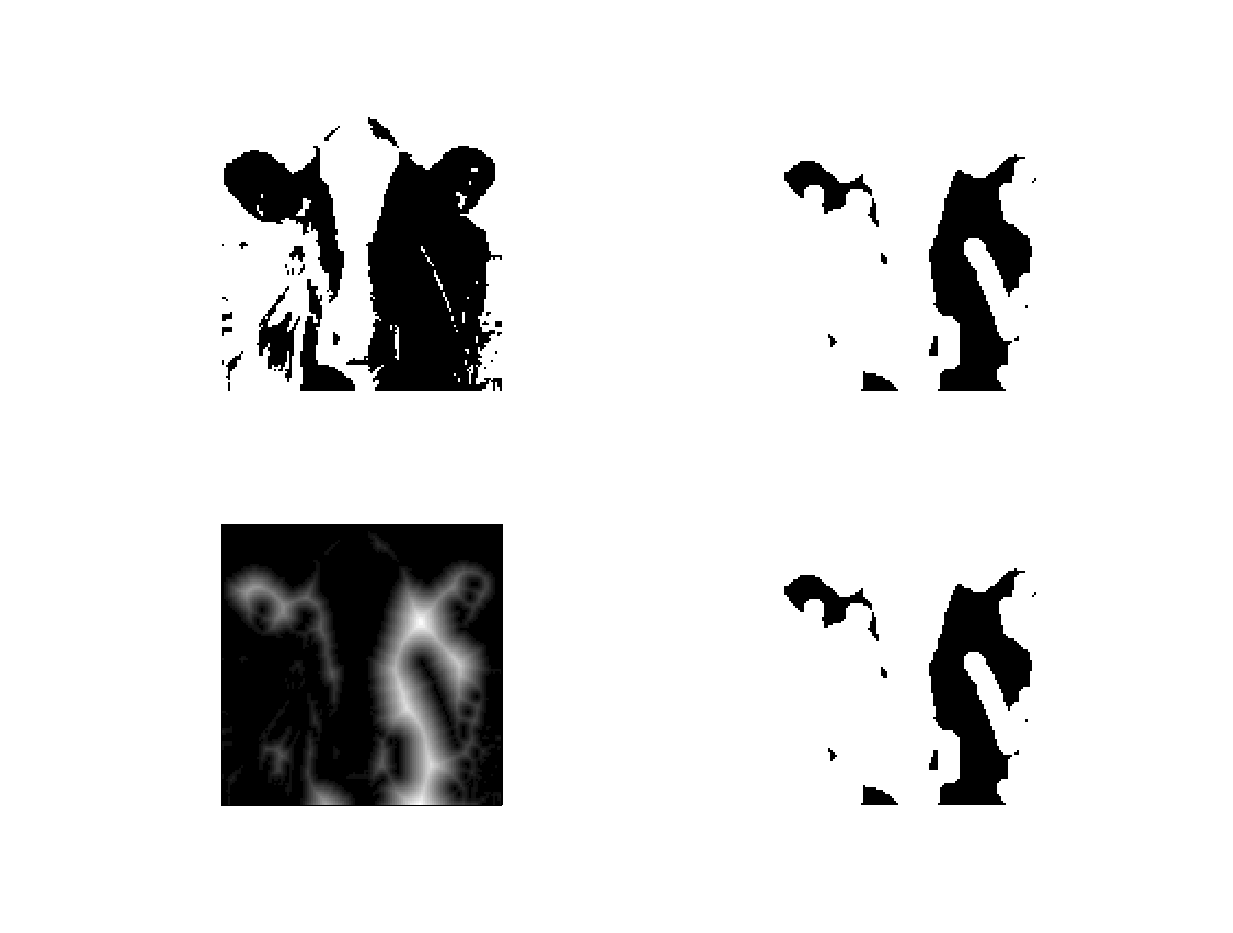
\includegraphics{data/tex/distanceAndDilatation-inc.eps}
\end{picture}%
\begin{picture}(576,432)(0,0)
\fontsize{10}{0}
\selectfont\put(165.6,396.743){\makebox(0,0)[b]{\textcolor[rgb]{0,0,0}{{Image originale}}}}
\fontsize{10}{0}
\selectfont\put(430.56,396.743){\makebox(0,0)[b]{\textcolor[rgb]{0,0,0}{{Image dilatee par une boule de rayon 5}}}}
\fontsize{10}{0}
\selectfont\put(118.831,48.5153){\makebox(0,0)[t]{\textcolor[rgb]{0,0,0}{{20}}}}
\fontsize{10}{0}
\selectfont\put(139.851,48.5153){\makebox(0,0)[t]{\textcolor[rgb]{0,0,0}{{40}}}}
\fontsize{10}{0}
\selectfont\put(160.871,48.5153){\makebox(0,0)[t]{\textcolor[rgb]{0,0,0}{{60}}}}
\fontsize{10}{0}
\selectfont\put(181.89,48.5153){\makebox(0,0)[t]{\textcolor[rgb]{0,0,0}{{80}}}}
\fontsize{10}{0}
\selectfont\put(202.91,48.5153){\makebox(0,0)[t]{\textcolor[rgb]{0,0,0}{{100}}}}
\fontsize{10}{0}
\selectfont\put(223.929,48.5153){\makebox(0,0)[t]{\textcolor[rgb]{0,0,0}{{120}}}}
\fontsize{10}{0}
\selectfont\put(93.355,167.529){\makebox(0,0)[r]{\textcolor[rgb]{0,0,0}{{20}}}}
\fontsize{10}{0}
\selectfont\put(93.355,146.509){\makebox(0,0)[r]{\textcolor[rgb]{0,0,0}{{40}}}}
\fontsize{10}{0}
\selectfont\put(93.355,125.49){\makebox(0,0)[r]{\textcolor[rgb]{0,0,0}{{60}}}}
\fontsize{10}{0}
\selectfont\put(93.355,104.47){\makebox(0,0)[r]{\textcolor[rgb]{0,0,0}{{80}}}}
\fontsize{10}{0}
\selectfont\put(93.355,83.4505){\makebox(0,0)[r]{\textcolor[rgb]{0,0,0}{{100}}}}
\fontsize{10}{0}
\selectfont\put(93.355,62.431){\makebox(0,0)[r]{\textcolor[rgb]{0,0,0}{{120}}}}
\fontsize{10}{0}
\selectfont\put(165.6,198.023){\makebox(0,0)[b]{\textcolor[rgb]{0,0,0}{{carte de distance}}}}
\fontsize{10}{0}
\selectfont\put(430.56,198.023){\makebox(0,0)[b]{\textcolor[rgb]{0,0,0}{{Seuillage de la carte de distance... dilatation}}}}
\end{picture}
